% Created 2013-05-23 Thu 09:29
\documentclass{article}
\usepackage{epcc}
\usepackage{hyperref}

\title{Sharpen Exercise: Outcomes Summary}
\author{Toni Collis}
\date{}
%\date{21 April 2014}  

\begin{document}

\makeEPCCtitle

This is an example set of results from the sharpen code running on
HECToR, the predecessor to ARCHER as the UK national
supercomputer. HECToR was very similar to ARCHER except that it had
more CPU-cores per node (32 on HECToR vs 24 on ARCHER).

A single node (32 cores) was used and each case repeated 5 times and
averaged to produce the final timings. Example answers to the
questions raised in the practical are included below.

\section{Experience Gained}
\label{sec-1}

Through this exercise you should have gained experience in the following:

\begin{itemize}
\item Accessing a remote HPC resource using SSH.
\item Using the command line to navigate the file tree and examine files.
\item Using the job submission system to:
\begin{itemize}
\item Run batch jobs using job submission scripts.
\end{itemize}
\item Assessing the performance and scaling properties of a parallel application.
\end{itemize}
\section{Timing Results}
\label{sec-2}


\subsection{Overall Run Time}
\label{sec-2.1}


These are the times for the ``Overall Run Time'' produced by the sharpen
program. This includes all parts of the application: initialisation,
input/output and calculation times. All times in seconds.


\begin{center}
\begin{tabular}{rrrrrrr}
 Cores  &     Time 1  &     Time 2  &     Time 3  &     Time 4  &     Time 5  &  Average Time  \\
\hline
     1  &  10.807072  &  10.654838  &  10.652846  &  10.709710  &  10.658892  &     10.696672  \\
     2  &   5.639540  &   5.852772  &   5.642984  &   5.673884  &   5.638595  &      5.689555  \\
     4  &   2.963334  &   2.969696  &   2.974003  &   2.963424  &   2.964110  &     2.9669134  \\
     8  &   1.711736  &   1.746570  &   1.710573  &   1.717299  &   1.710906  &     1.7194168  \\
    16  &   1.034717  &   1.019144  &   1.052394  &   1.021498  &   1.020104  &     1.0295714  \\
    32  &   0.778760  &   0.781110  &   0.794290  &   0.818504  &   0.778740  &     0.7902808  \\
\end{tabular}
\end{center}



\subsection{Calculation Time}
\label{sec-2.2}


These are the results for the ``Calculation Time'' produced by the
sharpen application. This only includes the computation time and none
of the initialisation, communications or input/output. All times in seconds.



\begin{center}
\begin{tabular}{rrrrrrr}
 Cores  &     Time 1  &     Time 2  &     Time 3  &     Time 4  &     Time 5  &  Average Time  \\
\hline
     1  &  10.625828  &  10.560966  &  10.560098  &  10.560715  &  10.560508  &     10.573623  \\
     2  &   5.517322  &   5.589415  &   5.517923  &   5.516653  &   5.517236  &     5.5317098  \\
     4  &   2.838534  &   2.844219  &   2.839195  &   2.838236  &   2.838451  &      2.839727  \\
     8  &   1.571196  &   1.571108  &   1.571592  &   1.571103  &   1.571307  &     1.5712612  \\
    16  &   0.888845  &   0.875638  &   0.907217  &   0.875720  &   0.875330  &       0.88455  \\
    32  &   0.567534  &   0.569485  &   0.568508  &   0.566492  &   0.567021  &      0.567808  \\
\end{tabular}
\end{center}



\section{Speedup Results}
\label{sec-3}


All speedups are calculated relative to the time taken when using 1
core. The plot of speedup vs number of CPU-cores used (the number of
parallel MPI tasks) is shown below and the full datasets are available
in the tables.
\ \\
\ \\
{\centerline{\resizebox{0.70\hsize}{!}{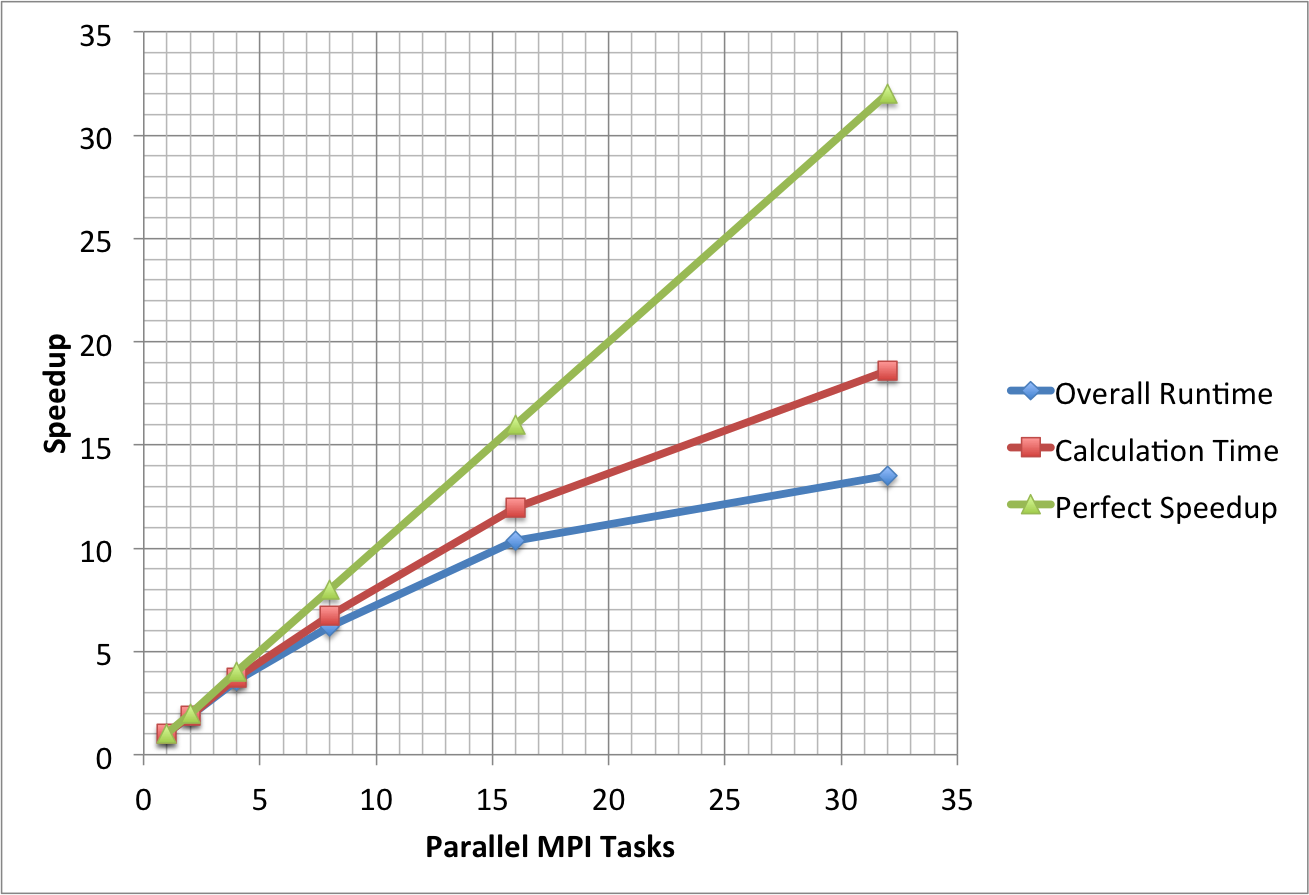
\includegraphics{sharpen_speedup.png}}}}

\subsection{Overall}

\begin{center}
\begin{tabular}{rrrrr}
 Cores  &  Average Time / s  &  Perfect Speedup  &    Speedup  &  \% of Perfect  \\
\hline
     1  &     10.696672  &              1.0  &         1.  &           100.  \\
     2  &      5.689555  &              2.0  &  1.8800542  &       94.00271  \\
     4  &     2.9669134  &              4.0  &  3.6053199  &      90.132998  \\
     8  &     1.7194168  &              8.0  &  6.2211047  &      77.763809  \\
    16  &     1.0295714  &             16.0  &  10.389442  &      64.934013  \\
    32  &     0.7902808  &             32.0  &  13.535280  &       42.29775  \\
\end{tabular}
\end{center}



\subsection{Calc}
\label{sec-3.2}


\begin{center}
\begin{tabular}{rrrrr}
 Cores  &  Average Time / s  &  Perfect Speedup  &    Speedup  &  \% of Perfect  \\
\hline
     1  &     10.573623  &              1.0  &         1.  &           100.  \\
     2  &     5.5317098  &              2.0  &  1.9114566  &       95.57283  \\
     4  &      2.839727  &              4.0  &  3.7234646  &      93.086615  \\
     8  &     1.5712612  &              8.0  &  6.7293859  &      84.117324  \\
    16  &       0.88455  &             16.0  &  11.953675  &      74.710469  \\
    32  &      0.567808  &             32.0  &  18.621828  &      58.193213  \\
\end{tabular}
\end{center}



\section{Example answers to questions}
\label{sec-4}



Q. What would the speedup be in each case if the code showed perfect
   scaling?

See tables above: in the perfect case, using double the number of
cores would halve the runtime of the application (2x speedup);
quadruple the number of cores would quarter the runtime (4x speedup);
\emph{etc.}


Q. How well is the code actually scaling?

The code gives >50\% of perfect scaling up to 16 cores for the overall
runtime which is reasonably good. If just the calculation time is
considered then the scaling is much improved. This indicates that as
the number of parallel tasks is increased then the serial components
of the code begin to dominate (for example, reading in the input and
writing out the output) leading to the poorer scaling seen for
overall runtime.


Q. What is the cheapest number of cores to use for this example
   (assuming that you are charged as walltime multiplied by number of
   cores)?

Just using a single core is the cheapest (and always will be unless
your speedup is better than perfect -- ``super-linear'' speedup). However, we are often
interested in the elapsed time as we may need to get results as soon
as possible. Also, it may not be possible to run on small numbers of
cores depending on how much memory you need.

{\bf Note:} on most high-end systems, nodes are not shared between
users. This means you are charged for all the CPU-cores on a node
regardless of whether you actually use them. Typically we would be
running on many hundreds of CPU-cores not a few tens, so the real
question in practice is: what is the optimal number of nodes to use?

Q. You may need more than one run at each core count to be able
to compute an average runtime for the plot to look sensible. Can you
think of any reason why this may be?


Performance can vary for a single run do to contention for shared
resources. As all the cases here are run on a single node (and single
nodes are not shared between users on HECToR) there is no contention
for off-node communications. However, there will be contention with
other users' jobs on the system for access to disk to read and write
files which could slow the application down.

You should see that the calculation time is much more stable than the
overall time, i.e. the IO time varies a lot (here by up to factor of
2).

\end{document}
